\documentclass[a4paper,10pt]{llncs}
\usepackage{fullpage}
\usepackage[british]{babel}
\usepackage[T1]{fontenc}
\usepackage{amsmath}
\usepackage{amssymb}
\usepackage[T1]{fontenc}
\usepackage[latin1]{inputenc} 
%\usepackage{amsthm} \newtheorem{theorem}{Theorem}
\usepackage{color}
\usepackage{float}



\usepackage{caption}
\DeclareCaptionFont{white}{\color{white}}
\DeclareCaptionFormat{listing}{\colorbox{gray}{\parbox{\textwidth}{#1#2#3}}}
\captionsetup[lstlisting]{format=listing,labelfont=white,textfont=white}


\usepackage{alltt}
\usepackage{listings}
 \usepackage{aeguill} 
\usepackage{dsfont}
%\usepackage{algorithm}
\usepackage[noend]{algorithm2e}
%\usepackage{algorithmicx}
\usepackage{subfig}
\lstset{% parameters for all code listings
	language=Python,
	frame=single,
	basicstyle=\small,  % nothing smaller than \footnotesize, please
	tabsize=2,
	numbers=left,
%	framexleftmargin=2em,  % extend frame to include line numbers
	%xrightmargin=2em,  % extra space to fit 79 characters
	breaklines=true,
	breakatwhitespace=true,
	prebreak={/},
	captionpos=b,
	columns=fullflexible,
	escapeinside={\#*}{\^^M}
}


% Alter some LaTeX defaults for better treatment of figures:
    % See p.105 of "TeX Unbound" for suggested values.
    % See pp. 199-200 of Lamport's "LaTeX" book for details.
    %   General parameters, for ALL pages:
    \renewcommand{\topfraction}{0.9}	% max fraction of floats at top
    \renewcommand{\bottomfraction}{0.8}	% max fraction of floats at bottom
    %   Parameters for TEXT pages (not float pages):
    \setcounter{topnumber}{2}
    \setcounter{bottomnumber}{2}
    \setcounter{totalnumber}{4}     % 2 may work better
    \setcounter{dbltopnumber}{2}    % for 2-column pages
    \renewcommand{\dbltopfraction}{0.9}	% fit big float above 2-col. text
    \renewcommand{\textfraction}{0.07}	% allow minimal text w. figs
    %   Parameters for FLOAT pages (not text pages):
    \renewcommand{\floatpagefraction}{0.7}	% require fuller float pages
	% N.B.: floatpagefraction MUST be less than topfraction !!
    \renewcommand{\dblfloatpagefraction}{0.7}	% require fuller float pages

	% remember to use [htp] or [htpb] for placement


\usepackage{fancyvrb}
%\DefineVerbatimEnvironment{code}{Verbatim}{fontsize=\small}
%\DefineVerbatimEnvironment{example}{Verbatim}{fontsize=\small}

\usepackage{url}
\urldef{\mailsa}\path|sharyari@gmail.com |    
\newcommand{\keywords}[1]{\par\addvspace\baselineskip
\noindent\keywordname\enspace\ignorespaces#1}


\usepackage{tikz} \usetikzlibrary{trees}
\usepackage{hyperref}  % should always be the last package

% useful colours (use sparingly!):
\newcommand{\blue}[1]{{\color{blue}#1}}
\newcommand{\green}[1]{{\color{green}#1}}
\newcommand{\red}[1]{{\color{red}#1}}

% useful wrappers for algorithmic/Python notation:
\newcommand{\length}[1]{\text{len}(#1)}
\newcommand{\twodots}{\mathinner{\ldotp\ldotp}}  % taken from clrscode3e.sty
\newcommand{\Oh}[1]{\mathcal{O}\left(#1\right)}

% useful (wrappers for) math symbols:
\newcommand{\Cardinality}[1]{\left\lvert#1\right\rvert}
%\newcommand{\Cardinality}[1]{\##1}
\newcommand{\Ceiling}[1]{\left\lceil#1\right\rceil}
\newcommand{\Floor}[1]{\left\lfloor#1\right\rfloor}
\newcommand{\Iff}{\Leftrightarrow}
\newcommand{\Implies}{\Rightarrow}
\newcommand{\Intersect}{\cap}
\newcommand{\Sequence}[1]{\left[#1\right]}
\newcommand{\Set}[1]{\left\{#1\right\}}
\newcommand{\SetComp}[2]{\Set{#1\SuchThat#2}}
\newcommand{\SuchThat}{\mid}
\newcommand{\Tuple}[1]{\langle#1\rangle}
\newcommand{\Union}{\cup}
\usetikzlibrary{positioning,shapes,shadows,arrows}

\pagestyle{empty}

\title{\textbf{Modelling the Suzuki-Kasami Algorithm\\ with the SPIN Model Checker}}

\author{Jonathan Sharyari}

\institute{Freie Universit{\"a}t Berlin, Computer Science Department\\
Takustra{\ss}e 9. 14195 Berlin, Germany\\
\mailsa
}
\begin{document}
\maketitle


\begin{abstract}
In 1985, Suzuki and Kasami presented two distributed algorithms for mutual exclusion. In this paper, the claim of mutual exclusion, deadlock and starvation freedom are tested using model checking techniques. Using the spin model checker, a counterexample to deadlock freedom was found for one of the algorithms, and a modification is proposed that guarantees deadlock freedom.
\end{abstract}


\section{Introduction}
Model checking is the process of automatically verifying the correctness of a system description with respect to its specifications, by examining a model corresponding to the system. The result of model checking is in general a certificate of correctness, or a counterexample showing why the specifications are not met.

There are many tools for model checking available, with different approaches to model checking and with different strengths and weaknesses. The SPIN Model checker (typically written Spin) is a widely used tool for model checking distributed and concurrent systems. The spin model checker was used mainly because both the tested pseudo code and the spin modelling language (promela) has a syntax close to that of C.


\subsection{Suzuki and Kasami's Algorithm}

The Suzuki/Kasami algorithm\cite{Suzuki} (henceforth abbreviated \textsc{ska}), is a distributed mutual exclusion-algorithm that requires at most N message exchanges for every mutual exclusion invocation between N computer nodes.

Each of the N nodes between which mutual exclusion is to be realized runs two processes P1 and P2. Each node has two local arrays RN and LN and a queue Q, all of which are accessible by P1 and P2.

The array RN holds the latest received \texttt{REQUEST} identifier for each other node. Similarly, LN holds the \texttt{REQUEST} identifier of the latest carried out \texttt{REQUEST} of all the other nodes, of which the node has been notified. Since the algorithm is distributed, the local arrays RN and LN are not the same for each node, and for each node represent only the information of which the node has been informed.
The local queue Q holds the nodes that are currently requesting the privilege, in the order the requests have been received.


When a node $node_i$ wants to enter its critical section with its main process P, it needs to have the \texttt{PRIVILEGE} to do so. In case the node already holds the privilege, it enters the critical section directly, without informing the other processes or updating the arrays RN and LN. Otherwise a \texttt{REQUEST(i, n)} message is sent to all other nodes, where i is the nodes identifier (index) and n is the \texttt{REQUEST} identifier.

A requesting node will wait until it receives a \texttt{PRIVILEGE} message, before accessing its critical section. When it is done, it updates its queue by appending all the nodes requesting, that are not already in the queue. Then, a \texttt{PRIVILEGE} is sent to the node first in Q, and that node is removed from the queue.

In process P2 \texttt{REQUEST(i,n)} messages are received. The array RN is updated, so that the corresponding entry RN[i] is set to n. If the node currently holding the \texttt{PRIVILEGE} is not itself waiting for the privilege, it will forward the \texttt{PRIVILEGE} to $node_i$ by sending a \texttt{PRIVILEGE(Q, LN)} message.

The pseudo-code proposed in the original paper is listed in appendix \ref{sec:ska}.

\subsection{Suzuki and Kasami's Modified Algorithm}
The \textsc{ska} algorithm has the disadvantage of \texttt{REQUEST} identifier numbers being unbounded. In a modified version of the \textsc{ska} algorithm (henceforth abbreviated \textsc{skam}), Suzuki and Kasami propose a slightly changes to the above algorithm in order to bound the \texttt{REQUEST} identifiers by a value L but with the cost of additional message exchanges.

In the \textsc{skam} algorithm a third process P3 is added to each node, and a new message type \texttt{REPLY}. When a node $n_1$ receives a \texttt{REQUEST} with the \texttt{REQUEST} identifier L from node $n_3$, it will send a \texttt{REPLY} message back to the sending node and set RN[3] to 0. The process P3 receives the \texttt{REPLY} messages and increments the variable \texttt{replyCount} (local to the node). The idea is that when a node has finished its L:th critical section, it must wait until a \texttt{REPLY} message has been received from all other processes before it can give the \texttt{PRIVILEGE} to the next process. The replies are thus a guarantee that all other processes have updated their RN-values to 0.

\begin{figure}[t]
\begin{center}
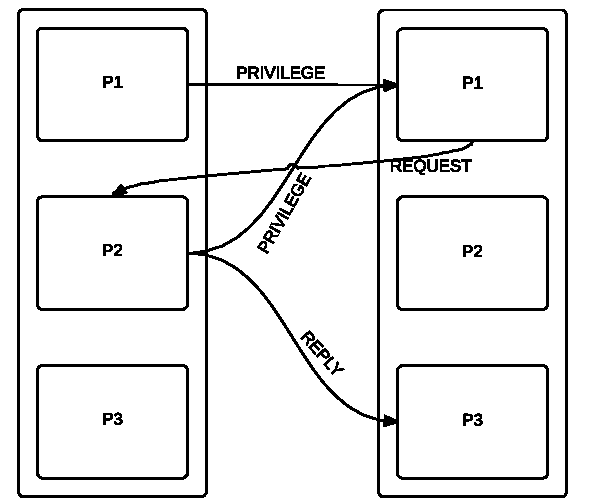
\includegraphics[width=0.55\textwidth]{Skaskam.pdf}
 \caption[Close up of \textit{Hemidactylus} sp.]
   {Two nodes running the \textsc{skam} algorithm, where the node to the left holds the privilege. The arrow heads point towards the receiver of the messages.}
\end{center}
\end{figure}



\section{Problem Formulation}
The \textsc{ska} and \textsc{skam} algorithms are claimed to guarantee mutual exclusion, starvation freedom and deadlock freedom. The purpose of this project is to investigate these claims and the additional property of being free from unnecessary delay, using model checking techniques. 

\section{Model of \textsc{ska} and \textsc{skam} in Promela}
Promela is a modelling language with a relatively small set of predefined types and function. Because of this, a model of the pseudo code in appendix \ref{sec:ska} must be implemented using the set of instructions available in promela.


\subsection{Nodes}
In the \textsc{ska} algorithm, every node has two processes which have shared variables. This style requires different levels of variable access, i.e. variables that can be accessed by several processes (meaning it is not local), but not by all processes (meaning it is not global). Since only global and local variables exist in promela, the model uses global variables for these shared variables. The global variables are seen perceived to belong to a node, and must only be accessed by processes within that node. To ensure this, every node has a node identifier, and every process is passed this identifier as an argument. 

The convention is, that for every shared variable, an array of those variables are created - one for each node. The $i$:th array cell belongs to node $i$, and is the only cell in the array that processes of node $i$ may access.

As an example, consider the boolean variable \texttt{requesting} belonging to node $i$, which must be accessible both by function P1(i) and P2(i). In promela, an array \texttt{requesting[N]} is created, and the processes may only access the cell \texttt{requesting[i]}.

\subsection{Queue}
A queue data structure could be implemented in several ways in promela, naturally suited for different applications. We note that in the \textsc{ska} algorithm, the key features of the queue is first that values are read \emph{first-in first-out} (FIFO) and second the ability to determine whether a certain value is already in the queue or not.

The promela channel data type is a FIFO data structure, but it provides no means of determining if a value is already in the queue or not. To surmount this problem, a new \emph{Queue} data structure is defined;

\begin{lstlisting}
typedef Queue {
  chan ch = [N] of {short};
  bool inQ[N];
}
\end{lstlisting}

This implementation draws upon the fact that a queue in this setting, needs at most store N values, since values may only be added if they are not already in the queue, and the range of numbers that are to be stored are the node indexes ranging from 0 to N-1.

To add a new value $n$ to the queue, it must first be checked that the value is already in the queue (\texttt{inQ[n]} is false). Then the value is added to the channel \texttt{ch}, and \texttt{inQ[n]} be set to true.

To remove the top value from the queue, the opposite is done. The value $n$ is read from the channel \texttt{ch}, and \texttt{inQ[n]} is set to false, indicating that the value $n$ is not in the queue.

\subsection{Messages}
Messages in promela can be sent using the built-in channel datatype (\texttt{chan}). There are different types of messages being sent, \texttt{PRIVILEGE}and REQUEST. To model this, new datatypes were defined as follows;

\begin{lstlisting}
typedef REQUEST{
  chan ch = [N] of {byte, byte};
}

typedef \texttt{PRIVILEGE}{
  chan ch = [N] of {Queue, Array};
}

\end{lstlisting}


In the model, a \texttt{REQUEST} is created for each node. When a node $i$ requests the \texttt{PRIVILEGE} with a \texttt{REQUEST} identifier $n$, it will write the values $(i,n)$ to the \texttt{REQUEST} channel of each process other than its own. As only one process has the \texttt{PRIVILEGE} at any time, only one instance of \texttt{PRIVILEGE} needs be created. When a node$i$ wants to send the \texttt{PRIVILEGE} to another node $j$, node $i$ will write its current Queue and its current LN-array to the \texttt{PRIVILEGE} channel.

Since the \texttt{PRIVILEGE} channel can be read by any node, there need be a way to determine which process is to read this channel. This is solved by a global array \texttt{havePrivilege[N]}, that is set to false for all indices except of that belonging to the current holder of the privilege. When the process $i$ above has sent its message on the channel, it will set \texttt (havePrivilege[i]) to false and \texttt (havePrivilege[j]) to true. This indicates to process $j$ that it can read the \texttt{PRIVILEGE} channel.

\texttt{REPLY} messages are implemented as a regular channel, writing and reading to the channel correspond to sending and receiving, and the values are of no importance.

\subsection{Event Handling}
The process P2 (and in \textsc{skam} also P3) is to be ran when a message is received. This indicates a type of event handler that does not exist in promela. To overcome this problem, we first note that the strength in using a event handler is that it does not rely on \emph{busy waiting}, i.e. a loop that continuously checks whether a certain predicate is true before it continues. In a classic programming language such a C, busy waiting requires much processing power. In promela though, an if-statement or a loop for which no predicate is true will always wait until the predicate is true without using busy waiting. This means that busy waiting in promela is not at all ``busy'', and therefore  process P2 can be implemented as a loop with the predicate \texttt{nempty(REQUESTING[i])}.

It is easy to see that the loop will be run once for each message received, and since Spin does not always execute the loop as soon as it is possible, arbitrarily long ``time'' may pass until a \texttt{REQUEST} is actually processed. On the other hand, messages can only be received in the order they are sent whereas in reality a message can be delayed without affecting other messages. To solve this issue, the loop can be extended with the non-deterministic choice of reading a message and write it back to the end of the queue, in effect delaying the message.


\section{Properties as LTL-Formulae}
Due to the \texttt{REQUEST} identifier numbers, the \textsc{ska} algorithm has the disadvantage of unboundedness, meaning that the state space of the model is infinite. There are techniques to overcome these problem, for example to only check the validity of properties within a finite portion of the infinite transition system. Another solution is to model an abstraction of the algorithm, in order to bound the state space (using the fact that the actual \texttt{REQUEST} number is not interesting, only whether it is smaller than some other value or not).

In this paper, the former approach was used to bound the searched portion of the transition system. The models were checked both for two and three processes running in parallell, and with the value of L set to 2 (in the \textsc{skam} model).

WHY CAN A MODEL WITH FOUR PROCESSES NOT EXHIBIT MORE BEHAVIOURS THAN A MODEL WITH THREE PROCESSES? DISKUSSION?

\subsection{Deadlock Freedom}
With the spin model checker, deadlocked states are considered to be erroneous states and are included in a standard set of checks run by spin. Thus no extra effort is required to determine the absence of such states, as it will be done automatically unless the model checker is not told to ignore invalid end states. Deadlock freedom can also be shown explicitly for the \textsc{skam} model by checking the LTL-formula \texttt{[]!timeout}. \texttt{timeout} is a predefined global read-only name in the promela language, and is true only if no active process is able to proceed.

The corresponding LTL-formula for the \textsc{ska} model simulating two nodes is
\texttt{!timeout U (RN[0].ind[0] > 2 || RN[1].ind[1] > 2)}.

Here \texttt{RN[0].ind[0]} denotes the value of RN[0] in the node with node identifier 0. This formula says that no deadlocks can occur, while the \texttt{REQUEST}numbers of all processes is less than 2.

\subsection{Starvation Freedom}
Starvation freedom is the property that no node is consistently over run by the other processes, i.e. every process will get its turn eventually. This is a liveness property, and needs some degree of fairness to be checked for situations that are reasonable. For example, a node that never requests to enter the critical section will never enter its critical section. Using fairness properties, this kind of irrelevant examples can be excluded. Fairness assumptions can easily be expressed in LTL, in particular it can be expressed that if a process $n_i$ wants to enter its critical section continuously (that is weak fairness), it will always be able to eventually: \texttt{<>[]requesting[i] -> []<>havePrivilege[i]}.

The corresponding LTL formula for the \textsc{ska} model simulating two processes is \texttt{(requesting[i] -> <>(havePrivilege[i])) U (RN[0].ind[0] > 2 || RN[1].ind[1] > 2)}. This formula says that if the node with node identifier i requests the privilege, it will eventually get the privilege, while the \texttt{REQUEST} numbers of all processes is less than 2. It is worth noting that expressed in this way, the property is no longer a liveness property but a safety property.


\subsection{Mutual Exclusion}
Mutual exclusion is the property that at most one node can be executing critical code at the same time. In promela, LTL formula can use built-in \emph{labels} to check properties such as \texttt{[]!(P1[0]@critSection \&\& P1[1]@critSection)}. Another way to check for mutual exclusion is to add a shared variable, which is increased by one each time a process enters the critical section, and decreased by one each time it leaves the critical section. The LTL formula to be checked is then \texttt{[]counter < 2}.

The corresponding LTL formula for the \textsc{ska} model simulating two processes is \texttt{(counter < 2) U (RN[0].ind[0] > 2 || RN[1].ind[1] > 2)}.

\subsection{Freedom of Unnecessary Delay}
\label{sec:delay}

This describes the property that a process that wishes to enter its critical section must not be delayed unless another process is already in the critical section. In contrast to the terms \emph{Starvation freedom} and \emph{deadlock} that are well-defined term, it is unclear what is to be considered ``Unnecessary'' delay. With a rigid definition of ``Unnecessary'', this property is trivially false - a token-based algorithm must at least wait for the token (i.e. the privilege). On the other hand, a too tolerant definition would make the property trivially true - if a process needs to wait at some point, then surely it is necessary to wait.

Let freedom of \emph{unnecessary delay} imply that when a node holds the privilege, it can enter the critical section without any additional communication with other nodes.

\section{Results}
\subsection{Deadlock Freedom}

\begin{figure}[]
\begin{center}
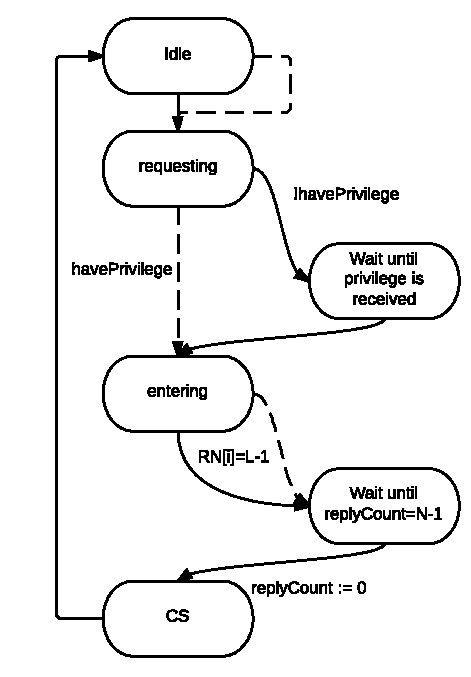
\includegraphics[width=0.5\textwidth]{Deadlock.pdf}
 \caption[Close up of \textit{Hemidactylus} sp.]
   {The behaviour of node $P1_n$ when a deadlock occurs. A continuous line marks a transition in the first iteration, a dashed line a transition in the second iteration. The example begins in the state \emph{idle}.}
\end{center}
\end{figure}

The \textsc{skam} algorithm was shown not to be free from deadlocks, but the deadlock is directly related to the modifications extending \textsc{ska} to \textsc{skam}, and would not be present in the \textsc{ska} algorithm. The problem can occur when a process $P1_n$ requests the \texttt{PRIVILEGE} for the L:th time; after receiving the \texttt{PRIVILEGE} process must wait additionally until the other processes have sent \texttt{REPLY}messages. The indicator of having received replies is a counter \texttt{replyCount}, which is set again to zero when the replies have been received. The deadlock can occur in the next iteration if none of the other processes have requested. If this happens, the process $P1_n$ can attempt to enter the critical section again, and does not need to increase increase its current \texttt{REQUEST} number. As the \texttt{REQUEST} number is unchanged, the process must again wait for the \texttt{REPLY} messages of the other processes, but these have already been sent and received. This marks a deadlock state, where the process holding the \texttt{PRIVILEGE} is waiting infinitely, and no other process can get the privilege. 

This problem can be solved rather simply, by adding a local variable \texttt{nreceived} to the process P1. The variable is set to 0 whenever a \texttt{REQUEST} is made, but said to 1 when all replies have been received. When the process P1 iterates again after its L:th request, it will only wait for replies if the indicator \texttt{nreceived} is not set.


\begin{figure}[]
\begin{center}
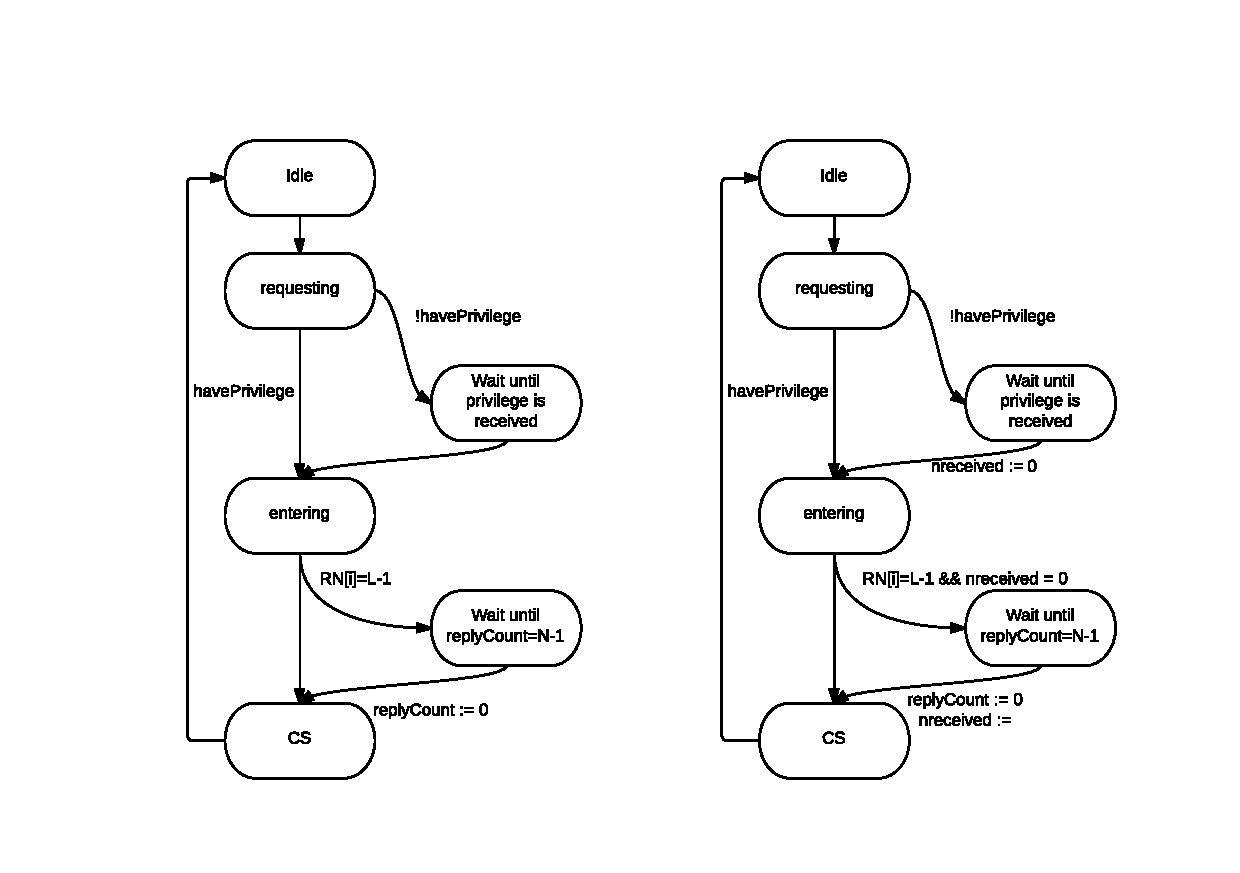
\includegraphics[width=\textwidth]{diagramboth.pdf}
 \caption[Close up of \textit{Hemidactylus} sp.]
   {Simplified flow chart of the \textsc{skam} algorithm (left). Flow chart after extending the model with a variable \texttt{nreceived}}
\end{center}
\end{figure}

Using this small extension the model was shown to be free from deadlocks. All further model checking results are based on the deadlock-free model. Note that it has been assumed that a nodes execute infinitely often (at least the node holding the privilege); without this non-termination assumption, a deadlock might occur  \cite{OgataSAL}\cite{OgataMaude}.

\subsection{Starvation Freedom and Mutual Exclusion}
The tests show that the \textsc{skam} algorithm satisfies mutual exclusion, and is free from starvation. The same results hold for \textsc{ska}, when checked in a bounded region of the transition system.

\subsection{Freedom of Unnecessary Delay}
As defined in \ref{sec:delay}, freedom of unnecessary delay implies that a node holding the \texttt{PRIVILEGE} may enter the critical section without any additional communication with other nodes. This property does not hold for the \textsc{skam} algorithm, since every L:th round the node with the \texttt{PRIVILEGE} must first wait for \texttt{REPLY} messages from the other nodes.

Promela provides the keyword \texttt{dstep}, which can be used to check this property. A block of code written within a \texttt{dstep} block must be executed deterministically; if the process must wait for a message to be received or for a condition to be true, the code is \emph{blocked}. In spin, a block within a \texttt{dstep} is perceived as an error. By enclosing the code following the point where the \texttt{PRIVILEGE} is received within a \texttt{dstep} block, this property can in effect be checked along side another property, for example while checking for starvation freedom.

The results show that the \textsc{ska} algorithm satisfies this property, and that the \textsc{skam} algorithm satisfies this property whenever the \texttt{REQUEST} identifier of a node is not L-1.

\section{Discussion}


\section{references}
\begin{thebibliography}{4}

\bibitem{OgataSAL}Ogata, K., Futatsugi, K.: Analysis of the Suzuki-Kasami Algorithm with SAL Model Checkers. In: 
Proceedings of the 2005 The Fifth International Conference on Computer and Information Technology (CIT 05)

\bibitem{OgataMaude} Ogata, K., Futatsugi, K.: Analysis of the Suzuki-Kasami Algorithm with the Maude Model Checker. In: 
Proceedings of the 12th Asia-Pacific Software Engineering Conference (APSEC 05)

\bibitem{Suzuki} Suzuki, I., Kasami, T.: A Distributed Mutual Exclusion Algorithm. In: 
ACM Transactions on Computer Systems, Vol. 3, No. 4, November 1985, Pages 344-349.


\end{thebibliography}

\appendix
\section{Appendix A}
\label{sec:ska}

\begin{lstlisting}[label=some-code,caption=Suzuki and Kazami's algorithm]
const I: Integer;		(* the identifier of this node *)
	var HavePrivilege, Requesting:		bool;
	j, n:	 	integer;
	Q: 		queue of integer;
	RN, LN:	array[l . . N] of integer;

	(* The initial values of the variables are:
	HavePrivilege= true in node 1, false in all other nodes;
	Requesting = false; Q = empty;
	RN[j] = -1, j = 1,2, . . . , N;  	LN[j] = -1, j = 1,2,. . . , N; *)

	procedure Pl;
	begin
		Requesting := true;
		if not HavePrivilege then
		begin
			RN[I] := RN[Z] + 1;
			for all j in 11, 2, . . . , NJ - {Z) do
				Send REQUEST(1, RN[I]) to node j;
			Wait until PRIVILEGE(Q, LN) is received;
			HavePrivilege:= true
		end,
	
		Critical Section;

		LN[Z] := RN[Z];
		for all j in 11, 2, . . . , N) - [I) do
			if not in(Q, j) and (RN[jJ = LN[j] + 1) then
				Q := append(Q, j);
		if Q f empty then
		begin
			HavePrivilege := false;
			Send PRIVILEGE(tail(Q), LN) to node head(Q)
		end;
		Requesting := false
	end,

	procedure P2; (* REQUEST(j,n) is received; P2 is indivisible *)
	begin
		RN[j] := max(RN[j],n);
		if HavePrivilege and not Requesting and (RN[j] = LN[j] + 1) then
		begin
			HavePrivilege:= false;
			Send PRIVILEGE(Q, LN) to node j
		end
	end,

\end{lstlisting}


\end{document}

